\chapter{Representaciones de color, hadrones y confinamiento}

\paragraph{Un breve interludio inicial.}
Antes de volver a la teoría de grupos, permítanme un descarado anuncio comercial. \emph{La guerra de los agujeros negros} cuenta la larga discusión con Stephen Hawking sobre si los agujeros negros destruyen la información cuántica. También relata una crueldad propia de los físicos teóricos: no solo el gato de Schrödinger, sino también el pez de Susskind y su desafortunado viaje por el retrete. Cumplido ese deber, volvamos a Alice y Bob. Alice sigue sufriendo, porque Bob todavía la obliga a aprender teoría de grupos.

\lectureoverview{Una simetría se vuelve física por medio de su acción sobre los estados. Empezaremos con las rotaciones para introducir las representaciones y los generadores; después repetiremos la construcción para el color \(SU(3)\). Las representaciones de color se combinan para formar hadrones, y su dinámica explica por qué nunca se observa color aislado.}

\section{El grupo y los objetos sobre los que actúa}

En toda discusión sobre simetrías hay dos ideas. Primero, un grupo abstracto: un conjunto de operaciones con una ley de multiplicación, un elemento identidad e inversos. Segundo, los objetos sobre los que actúan esas operaciones. Se pueden distinguir ambas ideas, pero en física no se pueden separar. Una simetría importa porque transforma estados físicos, campos, coordenadas u observables.

\begin{classroomqa}
\audiencequestion{Se ha descrito un grupo tanto como una tabla de multiplicación abstracta como mediante matrices que actúan sobre objetos físicos. ¿Se pueden disociar esas dos partes?
\lecturetimestamp{00:01:58}}
\lecturerresponse{Son niveles de descripción distintos, pero están completamente relacionados. Una rotación existe como operación abstracta antes de especificar qué rota. La física pregunta entonces cómo actúa esa misma operación sobre los estados y las magnitudes pertinentes para un sistema concreto. Las matrices proporcionan esa acción concreta y, a la vez, preservan la ley de multiplicación abstracta.}
\end{classroomqa}

Las rotaciones espaciales ofrecen el ejemplo más sencillo. En la mecánica clásica, una misma rotación puede actuar sobre las coordenadas de una partícula, sobre la dirección de un imán o sobre cualquier otro vector. En mecánica cuántica, los estados pertenecen a un espacio vectorial lineal, así que una rotación se representa mediante un operador lineal sobre ese espacio. Si \(g\) denota un elemento abstracto del grupo y \(D(g)\) su matriz representante, la consistencia exige que
\begin{equation}
D(g_1g_2)=D(g_1)D(g_2),
\qquad
D(e)=\boldsymbol 1.
\end{equation}
Las matrices no tienen por qué parecerse a las operaciones abstractas, pero su multiplicación debe reproducir la multiplicación del grupo.
\editorialnote{La ecuación de homomorfismo expresa explícitamente la correspondencia entre la multiplicación de grupo y la multiplicación de matrices que la fuente describe verbalmente.}

La dimensión de la matriz viene determinada por el espacio de estados, no solo por el grupo abstracto. Si conservamos únicamente el espín de un electrón, hay dos posibilidades ortogonales, espín hacia arriba y espín hacia abajo, y un estado es un vector columna de dos componentes. Por tanto, las rotaciones actúan mediante matrices \(2\times2\). Para dos objetos de espín un medio hay cuatro estados de base,
\begin{equation}
\ket{\uparrow\uparrow},\qquad
\ket{\uparrow\downarrow},\qquad
\ket{\downarrow\uparrow},\qquad
\ket{\downarrow\downarrow},
\end{equation}
y la acción inducida sobre el espacio combinado es tetradimensional.

La secuencia conocida es
\begin{equation}
\begin{array}{c|c|c}
\text{spin} & \text{number of states} & \text{matrix dimension}\\
\hline
0 & 1 & 1\times1\\
\frac12 & 2 & 2\times2\\
1 & 3 & 3\times3\\
\frac32 & 4 & 4\times4
\end{array}
\end{equation}
y así sucesivamente. Un estado de espín cero proporciona la representación trivial: toda rotación lo deja inalterado. La matriz de una por una es simplemente \(1\). Un estado de espín uno tiene tres componentes, y sus matrices de rotación son las conocidas rotaciones vectoriales tridimensionales. En general, el espín \(j\) tiene \(2j+1\) estados.

La representación también puede ser infinidimensional. Si describimos todo el movimiento orbital de un electrón, en lugar de solo su espín, el estado contiene una amplitud para cada posición o, de forma equivalente, para cada momento. El operador de rotación actúa entonces sobre un espacio infinidimensional de funciones de onda. Así pues, un mismo grupo abstracto de rotaciones tiene representaciones triviales, bidimensionales, tridimensionales e infinidimensionales. Este es el hecho que volveremos a utilizar cuando pasemos del espín al color.

\section{Por qué las rotaciones de espín son unitarias especiales}

Volvamos ahora al espín de un solo electrón y descartemos su movimiento orbital. Una rotación se representa mediante una matriz unitaria \(2\times2\)\(U\),
\begin{equation}
U^\dagger U=\boldsymbol 1,
\qquad
U^{-1}=U^\dagger.
\label{eq:l4-unitarity}
\end{equation}
La transformación inversa debe deshacer la rotación, y la unitariedad conserva la norma y, por tanto, todas las probabilidades.

Una matriz compleja \(2\times2\) general contiene cuatro elementos complejos, es decir, ocho parámetros reales. La ecuación~\eqref{eq:l4-unitarity} impone cuatro condiciones reales independientes, con lo que quedan cuatro parámetros. Una rotación espacial ordinaria solo tiene tres: dos parámetros fijan el eje y uno fija el ángulo. Por tanto, a la matriz unitaria le sobra una fase. La restricción adicional es
\begin{equation}
\det U=1.
\label{eq:l4-det-one}
\end{equation}
El recuento queda así:
\begin{equation}
8-4-1=3.
\end{equation}

La restricción de determinante uno se conserva al multiplicar, porque
\begin{equation}
\det(AB)=\det A\,\det B.
\end{equation}
Si dos matrices tienen determinante uno, también lo tiene su producto. Además, es compatible con la unitariedad. Al tomar el determinante de
la ecuación~\eqref{eq:l4-unitarity} se obtiene
\begin{equation}
1=\det(U^\dagger U)
=\det(U^\dagger)\det U
=(\det U)^*\det U.
\end{equation}
En consecuencia, el determinante de una matriz unitaria se encuentra en el círculo unidad:
\begin{equation}
\det U=e^{i\phi}.
\end{equation}

\begin{classroomqa}
\audiencequestion{¿La unitariedad exige que el determinante sea real?
\lecturetimestamp{00:12:10}}
\lecturerresponse{No. La unitariedad solo exige que su módulo sea uno. El determinante puede ser cualquier fase pura \(e^{i\phi}\). Para una matriz bidimensional, multiplicar \(U\) por \(e^{-i\phi/2}\) elimina esa fase común y produce una matriz de determinante uno.}
\end{classroomqa}

En efecto, si
\begin{equation}
V=e^{-i\phi/2}U,
\end{equation}
entonces \(V\) sigue siendo unitaria y
\begin{equation}
\det V=e^{-i\phi}\det U=1.
\end{equation}
Las matrices unitarias de determinante uno forman \(SU(2)\).

Hay un detalle sutil. Es tentador decir que \(SU(2)\) es simplemente el grupo de rotaciones en el espacio tridimensional, pero la correspondencia es dos a uno. Las matrices \(U\) y \(-U\) actúan de manera distinta sobre un espinor, aunque corresponden a la misma rotación de un vector ordinario. Por tanto,
\begin{equation}
SU(2)/\{\boldsymbol 1,-\boldsymbol 1\}\simeq SO(3).
\end{equation}
Para la discusión actual importan la estructura local de multiplicación y los tres generadores, pero el recubrimiento doble explica la doble valoración de las rotaciones de espín un medio.

\section{Transformaciones infinitesimales y sus generadores}

Una rotación finita se puede construir a partir de muchas rotaciones muy pequeñas. Un elemento del grupo cercano a la identidad se llama infinitesimal y, en un grupo conexo, conocer todas las direcciones infinitesimales basta para reconstruir las transformaciones finitas mediante multiplicaciones repetidas. Más importante aún para la física, los operadores que generan estas transformaciones infinitesimales son las magnitudes conservadas asociadas a la simetría.

Escribamos un elemento cercano a la identidad como
\begin{equation}
U=\boldsymbol 1+i\epsilon T,
\qquad |\epsilon|\ll1.
\label{eq:l4-infinitesimal-u}
\end{equation}
El factor \(i\) es una convención práctica. Al sustituir esta expresión en la condición de unitariedad y descartar los términos de orden \(\epsilon^2\), se obtiene
\begin{align}
(\boldsymbol 1+i\epsilon T)
(\boldsymbol 1-i\epsilon T^\dagger)&=\boldsymbol 1,
\\
i\epsilon(T-T^\dagger)&=0,
\\
T&=T^\dagger.
\label{eq:l4-hermitian-generator}
\end{align}
El generador es hermítico, como debe serlo un observable de la mecánica cuántica.

\begin{figure}[htbp]
\centering
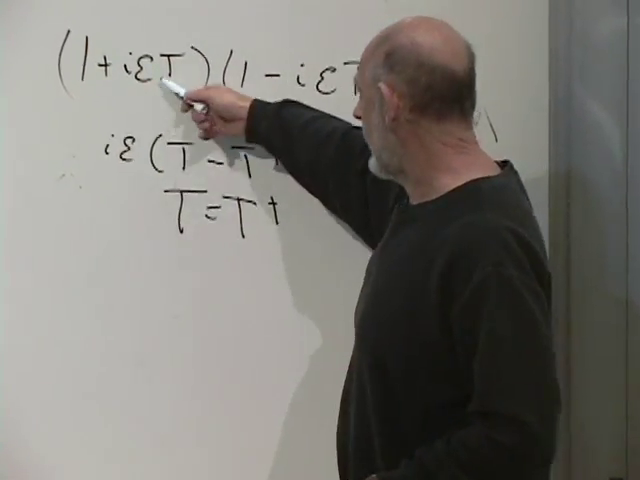
\includegraphics[width=0.62\textwidth]{lecture_04_figure_03.png}
\caption{Cálculo de la unitariedad cerca de la identidad, que termina en \(T=T^\dagger\).}
\lectureframe{00:23:28}
\end{figure}

Hay tres generadores linealmente independientes para las rotaciones espaciales, porque hay tres ejes infinitesimales independientes. Una rotación pequeña en una dirección arbitraria se construye mediante rotaciones pequeñas alrededor de \(x\), \(y\) y \(z\). Los generadores correspondientes son los operadores de momento angular \(J_x,J_y,J_z\). Sus conmutadores codifican la no conmutatividad de las rotaciones:
\begin{equation}
[J_i,J_j]=i\epsilon_{ijk}J_k.
\label{eq:l4-angular-momentum-algebra}
\end{equation}
Las rotaciones infinitesimales repetidas construyen entonces una rotación finita.

Hemos usado la unitariedad, pero todavía no la condición de determinante uno. Para cualquier matriz pequeña \(m\),
\begin{equation}
\det(\boldsymbol 1+\epsilon m)
=1+\epsilon\,\operatorname{tr}m+O(\epsilon^2).
\label{eq:l4-det-expansion}
\end{equation}

\begin{figure}[htbp]
\centering
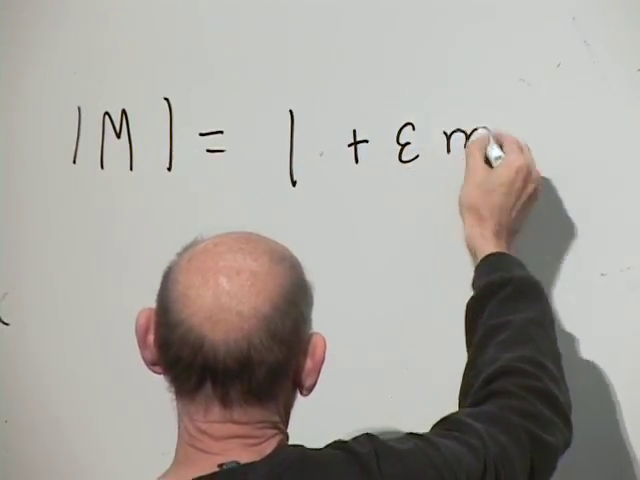
\includegraphics[width=0.62\textwidth]{lecture_04_figure_02.png}
\caption{Desarrollo del determinante a primer orden, tal como aparece al inicio en la pizarra.}
\lectureframe{00:21:51}
\end{figure}

Al aplicar la ecuación~\eqref{eq:l4-det-expansion} a la ecuación~\eqref{eq:l4-infinitesimal-u},
\begin{equation}
\det U
=1+i\epsilon\,\operatorname{tr}T+O(\epsilon^2).
\end{equation}
Por tanto, la condición de unitariedad especial exige que
\begin{equation}
\operatorname{tr}T=0.
\label{eq:l4-traceless-generator}
\end{equation}
Los generadores de \(SU(2)\) son precisamente las matrices hermíticas sin traza \(2\times2\). Ese espacio vectorial tiene dimensión tres. Las matrices de Pauli proporcionan una base estándar:
\begin{equation}
\begin{aligned}
\sigma_x&=
\begin{pmatrix}0&1\\1&0\end{pmatrix},
&
\sigma_y&=
\begin{pmatrix}0&-i\\i&0\end{pmatrix},
\\[0.4em]
\sigma_z&=
\begin{pmatrix}1&0\\0&-1\end{pmatrix}.
\end{aligned}
\end{equation}
Para una representación de espín un medio se puede tomar \(J_i=\sigma_i/2\), de modo que una rotación finita de ángulo \(\theta\) alrededor de \(\hat{\boldsymbol n}\) es
\begin{equation}
U(\hat{\boldsymbol n},\theta)
=\exp\!\left(-i\theta\,
\hat{\boldsymbol n}\cdot\boldsymbol\sigma/2\right).
\end{equation}
\editorialnote{La exponencial finita es la forma estándar de completar la discusión de los generadores infinitesimales. La fuente hace hincapié en las rotaciones pequeñas repetidas, en vez de escribir esta fórmula explícitamente.}

\begin{classroomqa}
\audiencequestion{¿Así que hay tres matrices hermíticas sin traza independientes \(2\times2\)?
\lecturetimestamp{00:24:07}}
\lecturerresponse{Sí. Son las tres matrices de Pauli. Para las matrices unitarias especiales \(3\times3\), el recuento correspondiente es ocho, y las ocho matrices de Gell-Mann forman una base convencional.}
\end{classroomqa}

\begin{classroomqa}
\audiencequestion{¿Ese ocho es el mismo ``ocho'' de la vía óctuple y los ocho gluones?
\lecturetimestamp{00:24:43}}
\lecturerresponse{Las matemáticas corresponden al mismo tipo de \(SU(3)\) teoría de representaciones, pero hay que especificar qué simetría \(SU(3)\) actúa. La simetría de sabor de la vía óctuple histórica no es el color \(SU(3)\). Los ocho gluones pertenecen a la representación adjunta del color \(SU(3)\).}
\end{classroomqa}

\section{De SU(2) al color SU(3)}

Ahora pasemos de matrices \(2\times2\) a matrices \(3\times3\). Una matriz compleja \(3\times3\) general tiene nueve elementos complejos, es decir, dieciocho parámetros reales. La condición \(U^\dagger U=\boldsymbol 1\) aporta nueve restricciones reales, y \(\det U=1\) impone una más. Por tanto,
\begin{equation}
18-9-1=8.
\end{equation}
Hay ocho direcciones infinitesimales independientes y ocho generadores hermíticos sin traza. A diferencia de \(SU(2)\), este grupo no es el grupo de rotaciones del espacio tridimensional ordinario. Es una simetría interna que actúa sobre el color.

Antes de asignar esas representaciones a los quarks, recordemos cómo surgen las representaciones compuestas. Pongamos juntos dos sistemas de espín un medio e ignoremos su movimiento orbital. Hay cuatro estados producto, pero una rotación no mezcla los cuatro de forma irreducible. Tres combinaciones se transforman como espín uno:
\begin{align}
\ket{1,1}&=\ket{\uparrow\uparrow},\\
\ket{1,0}&=\frac{1}{\sqrt2}
(\ket{\uparrow\downarrow}+\ket{\downarrow\uparrow}),\\
\ket{1,-1}&=\ket{\downarrow\downarrow},
\end{align}
mientras que la cuarta se transforma como espín cero:
\begin{equation}
\ket{0,0}=\frac{1}{\sqrt2}
(\ket{\uparrow\downarrow}-\ket{\downarrow\uparrow}).
\end{equation}
Así pues,
\begin{equation}
\boldsymbol 2\otimes\boldsymbol 2
=\boldsymbol 3\oplus\boldsymbol 1.
\label{eq:l4-two-spin-decomposition}
\end{equation}
Los estados alineados son los miembros \(m=\pm1\) del triplete; el estado simétrico de proyección cero lo completa, y la combinación antisimétrica es el singlete. Esta es la lógica general que subyace a la suma de momentos angulares y a la combinación de representaciones de color.

La misma distinción entre singlete--triplete aparece siempre que se acoplan dos grados de libertad de espín 1/2. En el hidrógeno atómico, los espines del electrón y del protón forman estados hiperfinos singlete y triplete. El ortohidrógeno y el parahidrógeno emplean la misma teoría de representaciones para los espines nucleares de los dos protones en una molécula de \(H_2\).\editorialnote{La fuente emplea ``ortohidrógeno y parahidrógeno'' al referirse a los espines protónicos--electrónicos de un átomo de hidrógeno. La descomposición matemática es correcta; aquí se distinguen los nombres moleculares y atómicos por precisión.}

\subsection{El triplete y el antitriplete}

Un quark tiene tres amplitudes de color. En una base elegida, escribamos
\begin{equation}
q=
\begin{pmatrix}
q_r\\q_g\\q_b
\end{pmatrix},
\qquad
q'=Uq,
\qquad U\in SU(3).
\label{eq:l4-quark-triplet}
\end{equation}
Las tres entradas pueden ser amplitudes de estado de un quark o tres operadores de campo que crean quarks rojos, verdes y azules. El grupo mezcla las tres componentes. Tras una transformación de color, un estado que inicialmente era rojo se convierte en general en una superposición de rojo, verde y azul. Esta representación fundamental tridimensional se llama \(\boldsymbol 3\).

Para un antiquark, el grupo actúa mediante la conjugada compleja de la representación del quark. Al tomar la conjugada compleja de la ecuación~\eqref{eq:l4-quark-triplet} se obtiene
\begin{equation}
\bar q'=U^*\bar q.
\end{equation}
Esta representación se denota \(\bar{\boldsymbol 3}\). La analogía con \(U(1)\) es inmediata: si un campo electrónico adquiere \(e^{i\theta}\), un campo de positrones adquiere \(e^{-i\theta}\). Las transformaciones de color de quarks y antiquarks constituyen la versión no abeliana de ese emparejamiento por conjugación.

Cerca de la identidad, si
\begin{equation}
U=\boldsymbol 1+i\epsilon T,
\end{equation}
entonces
\begin{equation}
U^*=\boldsymbol 1-i\epsilon T^*.
\end{equation}
Así pues, los generadores del antitriplete son \(-T^*\): los conjugados con el signo opuesto. Este es el sentido preciso en que los antiquarks tienen cargas de color opuestas.

\begin{classroomqa}
\audiencequestion{¿Qué ocurre con la representación conjugada compleja en el caso \(SU(2)\)?
\lecturetimestamp{00:36:19}}
\lecturerresponse{El doblete \(SU(2)\) es un caso especial: su conjugada compleja es equivalente al doblete original tras un cambio de base fijo que involucra el tensor épsilon antisimétrico. Para \(SU(3)\), en cambio, \(\boldsymbol 3\) y \(\bar{\boldsymbol 3}\) son representaciones genuinamente no equivalentes.}
\end{classroomqa}
\editorialnote{El término matemáticamente preciso para la representación fundamental de \(SU(2)\) es seudorreal, no real. La respuesta conserva la distinción que pretendía establecer la fuente y corrige la terminología.}

\section{Combinación de representaciones de color}

El símbolo \(\otimes\) no significa la multiplicación ordinaria de los números escritos junto a él. Significa que se combinan dos espacios de estados. El espacio producto tensorial resultante se reorganiza después en componentes que no se mezclan entre sí bajo la acción del grupo.

\subsection{Dos quarks: \texorpdfstring{\(\boldsymbol 3\otimes\boldsymbol 3\)}{3 x 3}}

Dos quarks tienen nueve estados de base de color: rojo--rojo, rojo--verde, rojo--azul y los seis pares ordenados restantes. Organicemos los dos índices de color en una parte simétrica y otra antisimétrica. La parte simétrica tiene seis componentes independientes; la antisimétrica tiene tres. Bajo \(SU(3)\),
\begin{equation}
\boldsymbol 3\otimes\boldsymbol 3
=\boldsymbol 6\oplus\bar{\boldsymbol 3}.
\label{eq:l4-three-times-three}
\end{equation}

\begin{figure}[htbp]
\centering
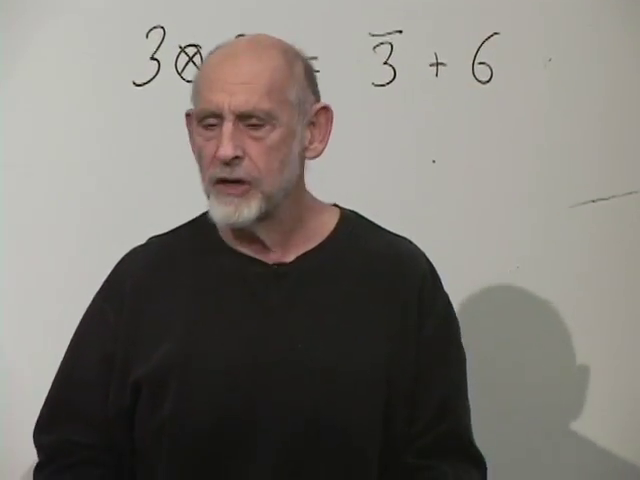
\includegraphics[width=0.68\textwidth]{lecture_04_figure_04.png}
\caption{Descomposición del producto de dos quarks en un antitriplete y un sextete.}
\lectureframe{00:39:33}
\end{figure}

El antitriplete se puede representar explícitamente contrayendo dos índices de quark con el tensor épsilon invariante:
\begin{equation}
(qq)^k_{\bar 3}
=\frac{1}{\sqrt2}\epsilon^{kij}q_iq_j.
\end{equation}
Este objeto tiene tres componentes y se transforma como un antiquark. Las seis combinaciones simétricas forman el sextete. No se afirma que dos quarks se conviertan dinámicamente en un antiquark, sino que un sector de su función de onda de color sigue la misma ley de transformación que un antiquark.

\subsection{Un quark y un antiquark: \texorpdfstring{\(\boldsymbol 3\otimes\bar{\boldsymbol 3}\)}{3 x anti-3}}

Un estado de color quark--antiquark se puede considerar una matriz \(3\times3\) \(M_i{}^j=q_i\bar q^j\). Toda matriz de este tipo se descompone de manera única en su parte de traza y su parte sin traza:
\begin{equation}
M=\frac{\operatorname{tr}M}{3}\boldsymbol 1
+\left(M-\frac{\operatorname{tr}M}{3}\boldsymbol 1\right).
\end{equation}
La traza es una única componente invariante, y la parte sin traza tiene ocho componentes. Por tanto,
\begin{equation}
\boldsymbol 3\otimes\bar{\boldsymbol 3}
=\boldsymbol 1\oplus\boldsymbol 8.
\label{eq:l4-three-times-threebar}
\end{equation}
El singlete, salvo por la normalización, es
\begin{equation}
\ket{1}_{q\bar q}
=\frac{1}{\sqrt3}
(\ket{r\bar r}+\ket{g\bar g}+\ket{b\bar b}).
\end{equation}
No puede rotar hacia ningún otro estado porque es invariante. Las otras ocho combinaciones lineales se mezclan entre sí. Constituyen la representación adjunta, la misma representación según la cual se transforman los ocho generadores.

\subsection{Tres quarks}

Combinemos un tercer quark con la ecuación~\eqref{eq:l4-three-times-three}. La rama del antitriplete da
\begin{equation}
\bar{\boldsymbol 3}\otimes\boldsymbol 3
=\boldsymbol 1\oplus\boldsymbol 8,
\end{equation}
Así, el producto de tres quarks contiene un singlete. En su forma completa,
\begin{equation}
\boldsymbol 3\otimes\boldsymbol 3\otimes\boldsymbol 3
=\boldsymbol 1\oplus\boldsymbol 8\oplus\boldsymbol 8
\oplus\boldsymbol{10}.
\label{eq:l4-three-quark-full}
\end{equation}
El singlete de color es la combinación totalmente antisimétrica rojo--verde--azul:
\begin{equation}
\ket{1}_{qqq}
=\frac{1}{\sqrt6}\epsilon^{ijk}\ket{q_iq_jq_k}.
\label{eq:l4-baryon-singlet}
\end{equation}
Como \(\epsilon^{ijk}\) se anula cuando dos índices coinciden, cada término no nulo contiene un quark rojo, uno verde y uno azul, con signos alternos al intercambiarlos.

\begin{classroomqa}
\audiencequestion{¿Son simplemente improbables las combinaciones no singlete, de modo que podemos ignorar sus probabilidades?
\lecturetimestamp{00:46:02}}
\lecturerresponse{No. El problema es la energía, no que la probabilidad sea pequeña. Un estado no singlete aislado tendría un campo de color que se extendería hasta distancias arbitrariamente grandes y, en el régimen de confinamiento, requeriría una energía ilimitada. Más adelante desarrollaremos la dinámica que sustenta esta afirmación.}
\end{classroomqa}

\subsection{El octeto de gluones}

El campo de gluones se transforma como el octeto de la ecuación~\eqref{eq:l4-three-times-threebar}. Respecto del color, lleva un índice de triplete y uno de antitriplete, y se elimina la traza singlete. Esquemáticamente,
\begin{equation}
q\sim\boldsymbol 3,
\qquad
\bar q\sim\bar{\boldsymbol 3},
\qquad
G\sim\boldsymbol 8.
\end{equation}
Estos símbolos indican leyes de transformación; las partículas no son literalmente iguales a los números tres y ocho.

La novena combinación de color quark--antiquark, proporcional a la identidad, es un singlete y no se mezcla con el octeto. Por tanto, es matemáticamente coherente omitirla: un campo gauge \(SU(3)\) no tiene traza y tiene ocho componentes, frente a las nueve de un campo gauge \(U(3)\).

\begin{classroomqa}
\audiencequestion{¿Por qué la naturaleza omite el gluón singlete adicional?
\lecturetimestamp{00:49:00}}
\lecturerresponse{La respuesta inmediata desde la teoría de grupos es que el singlete constituye un sector invariante separado, de modo que el octeto se cierra de manera consistente sin él. Aquí no se deriva la razón más profunda para elegir \(SU(3)\) en lugar de \(U(3)\); forma parte de la estructura gauge que se infiere de la fenomenología de la QCD.}
\end{classroomqa}

\section{Los singletes de color como hadrones}

Las partículas libres de masa finita de la interacción fuerte son singletes de color. Esto no significa que los quarks o los gluones no sean reales; significa que no aparecen como partículas asintóticas aisladas. Los patrones elementales para formar singletes son
\begin{equation}
qqq,
\qquad
q\bar q,
\qquad
GG\ \text{and higher gluonic products}.
\end{equation}
Dan lugar, respectivamente, a bariones, mesones y glueballs. Los productos de varios objetos ya neutros en color también son neutros, por supuesto, así que con estos componentes se pueden construir estados multihadrónicos más complejos.

\begin{classroomqa}
\audiencequestion{¿Cómo se llaman los singletes de tres quarks y de quark--antiquark, y también pueden los gluones formar singletes?
\lecturetimestamp{00:51:38}}
\lecturerresponse{Un singlete de tres quarks es un barión; un singlete de quark--antiquark es un mesón. Los gluones también pueden combinarse en singletes de color. Los estados más sencillos de este tipo que participan en la interacción fuerte se llaman glueballs, y pueden intervenir más de dos gluones.}
\end{classroomqa}

Tres quarks de espín un medio siempre se combinan para dar un espín total semientero, aunque el momento angular orbital puede cambiar cuál de ellos se obtiene. Los mesones de quark--antiquark tienen espín entero. Los glueballs puramente gluónicos también tienen espín entero.

La primera afirmación de la pizarra sobre dos gluones es solo un recuento:
\begin{equation}
8\times8=1+63.
\end{equation}
Hay sesenta y cuatro estados de color en total; una combinación es un singlete y los sesenta y tres restantes pertenecen a sectores no singlete.

\begin{figure}[htbp]
\centering
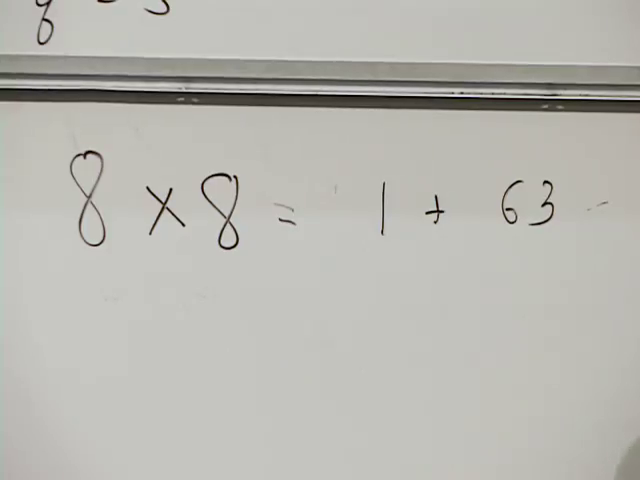
\includegraphics[width=0.68\textwidth]{lecture_04_figure_05.png}
\caption{Recuento de estados de dos gluones en la pizarra: un singlete entre sesenta y cuatro estados.}
\lectureframe{00:53:44}
\end{figure}

La descomposición irreducible completa es
\begin{equation}
\boldsymbol 8\otimes\boldsymbol 8
=\boldsymbol 1\oplus\boldsymbol 8_S\oplus\boldsymbol 8_A
\oplus\boldsymbol{10}\oplus\overline{\boldsymbol{10}}
\oplus\boldsymbol{27}.
\label{eq:l4-eight-times-eight}
\end{equation}
Las dimensiones suman correctamente:
\begin{equation}
1+8+8+10+10+27=64.
\end{equation}
Los dos octetos son subespacios invariantes distintos, uno simétrico y otro antisimétrico bajo el intercambio de los dos factores adjuntos. El singlete es el canal de color de dos gluones a partir del cual se puede formar un estado glueball.
\editorialnote{La pizarra da primero solo \(8\times8=1+63\). El intercambio posterior en clase proporciona las dimensiones irreducibles indicadas; aquí se restablecen las barras y las etiquetas de simetría con la notación estándar de \(SU(3)\).}

\subsection{Por qué las cargas eléctricas observables son enteras}

Las cargas de los quarks son de dos tipos:
\begin{equation}
Q_{\mathrm{up\text{-}like}}=+\frac23,
\qquad
Q_{\mathrm{down\text{-}like}}=-\frac13.
\end{equation}
Por tanto, tres quarks tienen una carga total entera: \(-1,0,+1,\text{ or }+2\), según cuántos sean del tipo up. Del mismo modo, un quark y un antiquark tienen carga \(0\) o \(\pm1\). Los gluones no tienen carga eléctrica. Así, los singletes de color básicos construidos con las representaciones de quarks observadas tienen carga eléctrica entera, aunque sus constituyentes tengan cargas fraccionarias.

\begin{classroomqa}
\audiencequestion{¿Cuál es la carga eléctrica del quark extraño?
\lecturetimestamp{00:56:08}}
\lecturerresponse{Es del tipo down, así que su carga es \(-1/3\). Las tres familias repiten el mismo patrón de cargas: \((u,d)\), \((c,s)\) y \((t,b)\), con cargas \(+2/3\) y \(-1/3\) en cada pareja.}
\end{classroomqa}

La condición de singlete de color y la carga eléctrica entera están estrechamente relacionadas para este contenido de partículas, pero no son afirmaciones matemáticas idénticas. La integridad también depende de las asignaciones concretas de carga eléctrica del modelo estándar que acabamos de escribir.

\begin{classroomqa}
\audiencequestion{¿Es un estado entrelazado un singlete de color, y tiene eso la misma importancia que una pareja entrelazada en un experimento de Bell?
\lecturetimestamp{00:56:58}}
\lecturerresponse{La función de onda del singlete de color sí está entrelazada: es una superposición coherente, no un producto de colores definidos por separado. En principio, sus constituyentes se pueden separar, pero el confinamiento hace que esa separación sea cada vez más costosa y, finalmente, produzca nuevos hadrones. Por eso no es un sistema práctico para una manipulación al estilo de Bell, aunque el estado esté entrelazado.}
\end{classroomqa}

\section{Qué significan las ecuaciones de producto tensorial}

En este punto, las tablas de multiplicación merecen una explicación más concreta. Sean \(\psi_i\) y \(\phi_j\) operadores que crean dos objetos de espín un medio; pueden describir dos especies, como un electrón y un protón, o dos copias de la misma especie cuando se tiene en cuenta la estadística apropiada. Cada índice toma dos valores. Los cuatro productos
\begin{equation}
\psi_\uparrow\phi_\uparrow,
\quad
\psi_\uparrow\phi_\downarrow,
\quad
\psi_\downarrow\phi_\uparrow,
\quad
\psi_\downarrow\phi_\downarrow
\end{equation}
generan el espacio producto tensorial.

Si un elemento del grupo actúa como \(U\) sobre cada factor, actúa como \(U\otimes U\) sobre el producto. En componentes,
\begin{equation}
\psi_i\phi_j
\longmapsto
U_i{}^kU_j{}^\ell\psi_k\phi_\ell.
\label{eq:l4-product-action}
\end{equation}
Esta es una representación tetradimensional, pero reducible. La combinación antisimétrica
\begin{equation}
\frac{1}{\sqrt2}
(\psi_\uparrow\phi_\downarrow
-\psi_\downarrow\phi_\uparrow)
\end{equation}
se transforma en sí misma, mientras que las tres combinaciones simétricas se transforman entre sí. En la base adaptada a esas combinaciones, todas las matrices de la representación producto adoptan una forma diagonal por bloques:
\begin{equation}
D_{2\otimes2}(g)
\sim
\begin{pmatrix}
1&0\\
0&D_3(g)
\end{pmatrix}.
\label{eq:l4-spin-block-diagonal}
\end{equation}

\begin{classroomqa}
\audiencequestion{¿Qué operación representa una ecuación como \(\boldsymbol 3\otimes\boldsymbol 3=\bar{\boldsymbol 3}\oplus\boldsymbol 6\)?
\lecturetimestamp{00:57:51}}
\lecturerresponse{El miembro izquierdo forma el espacio de estados compuesto. El grupo actúa sobre ambos factores y, por tanto, mezcla los estados de la base producto. El miembro derecho indica que un cambio de base separa esos estados en conjuntos invariantes: tres combinaciones antisimétricas que se transforman como un antitriplete y seis combinaciones simétricas que se transforman como un sextete. El signo más indica una suma directa de alternativas, no una suma numérica ordinaria.}
\end{classroomqa}

\begin{classroomqa}
\audiencequestion{¿Cómo sabemos que los nueve estados se descomponen como \(3+6\), o como \(1+8\), en lugar de, por ejemplo, como \(2+7\)?
\lecturetimestamp{01:04:39}}
\lecturerresponse{El recuento de dimensiones por sí solo no permite decidir la descomposición. Hay que saber qué representaciones irreducibles contiene \(SU(3)\) y construir subespacios invariantes, por ejemplo, simetrizando o antisimetrizando índices, o separando las partes con traza y sin traza. Una clasificación completa requiere más teoría de grupos; aquí solo usamos las representaciones necesarias para los quarks y los gluones.}
\end{classroomqa}

El tensor épsilon invariante hace transparente la construcción del singlete. Para \(SU(2)\),
\begin{equation}
\epsilon_{ij}U^i{}_kU^j{}_\ell
=(\det U)\epsilon_{k\ell}
=\epsilon_{k\ell}.
\end{equation}
Por tanto, \(\epsilon_{ij}\psi^i\phi^j\) es invariante. Para \(SU(3)\), la versión con tres índices da
\begin{equation}
\epsilon_{ijk}U^i{}_aU^j{}_bU^k{}_c
=(\det U)\epsilon_{abc}
=\epsilon_{abc},
\end{equation}
lo que demuestra la invariancia del estado de tres quarks de la ecuación~\eqref{eq:l4-baryon-singlet}.

\begin{classroomqa}
\audiencequestion{¿Se puede mostrar explícitamente por qué el singlete no se transforma?
\lecturetimestamp{01:07:18}}
\lecturerresponse{Sí. Contraigamos todos los índices fundamentales con el tensor épsilon totalmente antisimétrico. Bajo la transformación, el producto de matrices multiplica épsilon por \(\det U\). Para una matriz unitaria especial, ese determinante es uno, así que el estado contraído no cambia. En \(SU(2)\) esto demuestra la invariancia del singlete de dos espines; en \(SU(3)\) demuestra la del singlete de tres quarks rojo--verde--azul.}
\end{classroomqa}

\begin{classroomqa}
\audiencequestion{¿Cuál es la descomposición completa de dos octetos de gluones?
\lecturetimestamp{01:09:24}}
\lecturerresponse{Es la descomposición de la ecuación~\eqref{eq:l4-eight-times-eight}: un singlete, dos octetos, un decuplete, un antidecuplete y una representación de dimensión veintisiete. Hay exactamente una combinación de singlete de color de los dos índices de octeto.}
\end{classroomqa}

\begin{classroomqa}
\audiencequestion{¿Cuál es la descomposición completa correspondiente para tres quarks?
\lecturetimestamp{01:11:51}}
\lecturerresponse{La respuesta esencial desde el punto de vista físico es que contiene un singlete. Al completar el recuento se obtiene la ecuación~\eqref{eq:l4-three-quark-full}: un singlete, dos octetos y un decuplete, para un total de \(1+8+8+10=27\) estados.\editorialnote{Durante el intercambio, el profesor no recuerda la descomposición completa de \(3\otimes3\otimes3\). Aquí se proporciona explícitamente la descomposición estándar y se señala que no formó parte de la respuesta oral.}}
\end{classroomqa}

La misma idea se extiende al espacio de dos gluones. En la base producto ingenua,
\(SU(3)\) actúa mediante matrices \(64\times64\). En una base adaptada a las componentes irreducibles, esas matrices son diagonales por bloques,
\begin{equation}
\begin{aligned}
D_{8\otimes8}(g)
&\sim
\operatorname{diag}\bigl(
1,D_{8_S}(g),D_{8_A}(g),
\\
&\hspace{4.8em}
D_{10}(g),D_{\overline{10}}(g),D_{27}(g)
\bigr).
\end{aligned}
\end{equation}
Ningún bloque se mezcla con otro, aunque los estados de cada bloque sí se mezclan entre sí.

\begin{classroomqa}
\audiencequestion{¿La descomposición en productos tensoriales es simplemente un cambio a una base en la que la matriz grande de la representación queda diagonal por bloques?
\lecturetimestamp{01:12:02}}
\lecturerresponse{Exactamente. Para dos espines, la matriz de dimensión cuatro se convierte en un bloque singlete unidimensional y otro triplete de dimensión tres. Para dos gluones, la matriz de dimensión sesenta y cuatro se convierte en bloques de dimensiones \(1,8,8,10,10,\text{ and }27\). Cada bloque es cerrado bajo toda transformación del grupo.}
\end{classroomqa}

\begin{classroomqa}
\audiencequestion{¿Hay un nombre para una de esas partes cerradas dentro del espacio producto tensorial completo?
\lecturetimestamp{01:14:55}}
\lecturerresponse{Es un subespacio invariante que lleva una subrepresentación. Cuando no puede descomponerse más, lleva una representación irreducible, o irrep. El producto tensorial completo es la suma directa de esas componentes irreducibles.\editorialnote{En la fuente, el término solicitado queda sin resolver en el aula. La respuesta aporta la terminología estándar de la teoría de representaciones.}}
\end{classroomqa}

\begin{classroomqa}
\audiencequestion{Cuando se dice que los decupletes no singletes y otras representaciones no existen, ¿significa que deben ignorarse por completo?
\lecturetimestamp{01:15:36}}
\lecturerresponse{Son sectores de color legítimos e importan en los cálculos intermedios, pero no aparecen como partículas aisladas de energía finita en el laboratorio. Es el confinamiento, y no un fallo de la teoría de representaciones, lo que impide que se conviertan en estados asintóticos libres.}
\end{classroomqa}

\section{De la idea del color de Nambu al confinamiento}

La idea del color precede a la formulación definitiva de la QCD. Ya a principios de los años 1960, Yoichiro Nambu comprendió que un número cuántico oculto con tres valores podía resolver un problema sorprendente: los quarks tienen carga eléctrica fraccionaria, pero no se observan partículas libres con carga fraccionaria. Si se obliga a que los estados físicos sean singletes de color, los quarks aparecen en las combinaciones de carga entera descritas anteriormente. Queda la cuestión dinámica: ¿qué fuerzas hacen que todos los estados libres de energía finita sean singletes?

Empecemos con la analogía electromagnética. Una carga y otra de signo opuesto se atraen. Al acercarlas, disminuye la energía; juntar cargas del mismo signo requiere trabajo. El propio campo almacena energía positiva,
\begin{equation}
E_{\mathrm{field}}
=\frac12\int d^3x\,\boldsymbol E^2
\end{equation}
en unidades electrostáticas simples. Una carga neta deja un campo que se extiende mucho más allá del sistema, mientras que un par neutro estrechamente ligado solo tiene un campo dipolar de corto alcance. Por tanto, la neutralización elimina la energía del campo exterior.

Imaginemos que aumentamos enormemente el acoplamiento electromagnético. La penalización energética del campo por tener carga neta sería tan grande que los objetos de baja energía serían abrumadoramente neutros, y extraer un constituyente cargado podría resultar prohibitivamente costoso. Nambu trasladó esta intuición al color: las ocho cargas de color son fuentes de ocho campos gluónicos, así que una energía grande del campo de color podría impedir la existencia de estados no singletes aislados.

Esa intuición es esencialmente correcta, pero la QCD presenta una característica nueva decisiva. El fotón no tiene carga eléctrica, mientras que el gluón tiene carga de color. El fotón no es fuente del campo electromagnético clásico, y las ecuaciones de Maxwell son lineales: dos ondas electromagnéticas se superponen y atraviesan una a otra. El gluón se transforma según el octete de color, así que los gluones son fuentes e interactúan con otros gluones. Incluso distintas partes de un mismo campo gluónico interactúan entre sí. Por tanto, el campo de gauge no abeliano es no lineal.

\subsection{Tubos de flujo y potencial lineal}

A grandes distancias, la auto-interacción de los gluones impide que el flujo de color se disperse como un campo dipolar eléctrico ordinario. El flujo queda confinado en un tubo que une un quark con un antiquark. La intensidad del campo y el área de la sección transversal de un tubo largo son aproximadamente constantes, por lo que el tubo almacena una energía aproximadamente constante por unidad de longitud. Si \(\sigma\) denota esta tensión de cuerda, entonces
\begin{equation}
V(R)\simeq\sigma R+\text{constant}
\qquad (R\ \text{large}).
\label{eq:l4-linear-potential}
\end{equation}

\begin{figure}[htbp]
\centering
\includegraphics[width=0.78\textwidth]{lecture_04_figure_06.png}
\caption{Flujo de color agrupado en un tubo largo entre un quark y un antiquark.}
\lectureframe{01:31:35}
\end{figure}

Esto es más intenso que el potencial de Coulomb, cuya magnitud disminuye como \(1/R\).
Al separar más las fuentes de color, la fuerza no se debilita indefinidamente: el tubo se alarga y sigue acumulando energía. Una carga de color aislada en un volumen infinito requeriría un tubo sin fin y, por tanto, energía ilimitada. Este es el significado operativo de afirmar que solo los singletes de color tienen estados asintóticos de energía finita.
\editorialnote{La notación de la tensión de cuerda y el potencial explícito a grandes distancias cuantifican la afirmación de la fuente de que un tubo de flujo uniforme tiene una energía uniforme por unidad de longitud.}

\subsection{Ruptura de cuerdas y chorros}

Supongamos que una colisión de alta energía golpea un quark dentro de un mesón. El quark empieza a alejarse, pero el tubo de flujo se estira detrás de él. Puede perder energía cinética y ser arrastrado de vuelta. Con más frecuencia, cuando la energía almacenada en el campo es suficientemente grande, el vacío produce un nuevo par quark--antiquark. El nuevo antiquark termina el flujo unido al quark que escapa, mientras que el nuevo quark termina el flujo unido al antiquark original. Un singlete estirado se convierte en dos singletes más cortos,
\begin{equation}
(q\bar q)_{\mathrm{stretched}}
\longrightarrow
(q\bar q)+(q\bar q).
\label{eq:l4-string-breaking}
\end{equation}

\begin{figure}[htbp]
\centering
\includegraphics[width=0.78\textwidth]{lecture_04_figure_07.png}
\caption{La creación de pares rompe un tubo de flujo estirado en dos tubos singletes de color.}
\lectureframe{01:34:52}
\end{figure}

\begin{classroomqa}
\audiencequestion{Si un quark golpeado tiene suficiente energía para seguir estirando el tubo, ¿qué puede ocurrir además de que lo arrastren de vuelta?
\lecturetimestamp{01:33:50}}
\lecturerresponse{El tubo puede romperse mediante la creación de un par quark--antiquark. Su energía se convierte en la masa y la energía cinética del nuevo par. Los extremos se reconectan formando dos singletes, de modo que el proceso crea mesones adicionales en lugar de un quark aislado.}
\end{classroomqa}

Si uno de esos partones todavía tiene un momento grande, el proceso se repite. El resultado es una cascada de hadrones singletes de color, colimados alrededor de la dirección del partón original: un chorro. Esta conversión de quarks y gluones energéticos en hadrones se denomina hadronización. El objeto coloreado que inicia el proceso se infiere a partir del chorro; nunca se observa por sí solo.

\begin{classroomqa}
\audiencequestion{¿La ruptura de cuerdas produce únicamente mesones o también pueden aparecer otros hadrones en el chorro?
\lecturetimestamp{01:35:20}}
\lecturerresponse{Desde luego, también pueden aparecer otros hadrones. El único requisito de color es que los objetos observables finales sean singletes. Los mesones son la imagen más sencilla para una ruptura, pero también pueden producirse bariones, antibariones y combinaciones singletes más complejas.}
\end{classroomqa}

Tres quarks pueden terminar sus líneas de flujo en una unión singlete de color. La imagen de tres ramificaciones es la contraparte dinámica del tensor epsilon antisimétrico de la ecuación~\eqref{eq:l4-baryon-singlet}: no escapa flujo neto de color del barión completo.

\begin{figure}[htbp]
\centering
\includegraphics[width=0.72\textwidth]{lecture_04_figure_08.png}
\caption{Una unión de flujo de color con tres ramificaciones para un barión, debajo del esquema de ruptura de la cuerda del mesón.}
\lectureframe{01:36:12}
\end{figure}

\section{Campos de gauge, cargas conservadas y modelo estándar}

En el nivel actual, podemos reconocer una teoría de gauge como una teoría en la que una carga conservada es fuente de un campo análogo al del fotón. La carga eléctrica es fuente del campo electromagnético; las ocho cargas de color son fuentes de los ocho campos gluónicos. La formulación más profunda hace local la simetría e introduce una conexión que compara los estados internos en puntos vecinos del espacio-tiempo, pero esa construcción no hace falta para la explicación del confinamiento que desarrollamos aquí.
\editorialnote{La formulación mediante simetría local es el sentido más profundo y estándar de teoría de gauge al que alude la fuente, pero que deja deliberadamente para más adelante.}

La simetría, la carga conservada y el flujo están estrechamente relacionados. Si las líneas de campo solo pueden terminar en cargas, una fuente no puede desaparecer sin más mientras su flujo siga unido a algo. Tampoco puede desaparecer instantáneamente todo su campo distante, porque los cambios del campo se propagan causalmente. En su forma local, la misma física se expresa mediante una ecuación de continuidad,
\begin{equation}
\frac{\partial\rho}{\partial t}
+\boldsymbol\nabla\cdot\boldsymbol j=0,
\end{equation}
que establece que una carga solo puede salir de una región si fluye a través de su frontera. El argumento de las líneas de campo es la representación geométrica de esa ley local de conservación.

Ahora podemos situar este resultado dentro del modelo estándar. El color aporta los ocho generadores de \(SU(3)\) y sus ocho campos gluónicos. El sector abeliano aporta un generador y un campo de gauge. Otros tres generadores pertenecen a un \(SU(2)\) adicional, no al momento angular espacial ordinario. Antes de la ruptura de simetría, la estructura de gauge es
\begin{equation}
SU(3)_c\times SU(2)_L\times U(1)_Y,
\end{equation}
con \(8+3+1=12\) generadores. La siguiente tarea es comprender el sector electrodébil \(SU(2)\) y, después, el campo de Higgs y cómo aparecen el fotón observado, \(W^\pm\) y \(Z\).
\editorialnote{La fuente cuenta el fotón junto con los ocho gluones y describe el factor restante como \(SU(2)\times U(1)\). En el modelo estándar sin ruptura, el factor abeliano es la hipercarga \(U(1)_Y\); el fotón aparece solo después de la mezcla electrodébil.}

La cadena central está ahora completa. Los grupos abstractos actúan mediante representaciones; los generadores infinitesimales son las cargas conservadas; los quarks, antiquarks y gluones pertenecen a \(\boldsymbol 3\),
\(\bar{\boldsymbol 3}\) y \(\boldsymbol 8\), respectivamente; los productos tensoriales identifican los hadrones singletes; y el campo gluónico no lineal convierte la selección de singletes en el fenómeno físico del confinamiento.
